\section{Exercises from Lecture 5}

%%%%%%%%%%%%%%%%%%%%%%%%%%%%%%%%%%%%%%%%%%%%%%%%%%%%%%%%%%%%%%%%%%%%
\subsection{Exercise 5.4}

\emph{Prove the lemma: if $a + \varepsilon \geq b$ for arbitrary $\varepsilon > 0$ with $a, b \in \mathbb{R}$, then $a \geq b$.}
\\
\\
\textbf{Solution:}\\
\\
We can prove this by contradiction. We assume $a < b$ and arbitrarily choose $\varepsilon = \frac{b-a}{2}$. By hypothesis, we have

\begin{equation}
    a + \frac{b-a}{2} \geq b \iff \frac{a}{2} \geq \frac{b}{2} \iff a \geq b
\end{equation}

which contradicts our assumption. Hence, $a \geq b$.
\QEDB

%%%%%%%%%%%%%%%%%%%%%%%%%%%%%%%%%%%%%%%%%%%%%%%%%%%%%%%%%%%%%%%%%%%%
\subsection{Exercise 5.5}
\emph{Complete the proof of the principle of optimality by showing the reverse inequality $V(t,x) \leq \Bar{V}(t,x)$.}
\\
\\
\textbf{Solution:}\\
\\
After defining 
\begin{equation}
    \overline{V}(t,x) := \inf_{u[t, t+\Delta t] \to U} \left( \int_t^{t + \Delta t} L(s, x(s), u(s))ds + V(t + \Delta t, x(t + \Delta t)) \right)
\end{equation}

We have shown that $V(t,x) \geq \overline{V}(t,x)$. We can finish the proof of the equality by proving that $V(t,x) \leq \overline{V}(t,x)$  By definition of the value function, we have:
\begin{equation}
    V(t,x) := \inf_{u:[t, t_1]\to U, u \in V} J(t,x,u)
\end{equation}

From the previous results, we can continue the chain of inequalities:
\begin{align}
    \overline{V}(t,x) &= \int_t^{t + \Delta t} L(s, x_{\varepsilon}, u_\varepsilon(s))ds + \inf_{u:[t + \Delta t, t_1] \to U } J(t+ \Delta t, x_\varepsilon (t + \Delta t), u)\\
    &\geq \inf_{u:[t, t_1] \to U \in V} \int_t^{t + \Delta t} L(s, x_{\varepsilon}, u_\varepsilon(s))ds + \int_{t+\Delta t}^{t_1} L(s, x_{\varepsilon}, u_\varepsilon(s))ds + K(t_1, x_{\varepsilon})\\
    %&\text{since } L(s, x_{\varepsilon}, u_\varepsilon(s))ds \text{ does not depend on 
    &= \inf_{u:[t, t_1] \to U \in V} \int_t^{t_1} L(s, x_{\varepsilon}, u_\varepsilon(s))ds + K(t_1, x_{\varepsilon})\\
    &= \inf_{u_\varepsilon:[t, t_1] \to U, u \in V} J(t, x, u)\\
    &= V(t, x)
\end{align}
Thus, we have shown that $V(t,x) \leq \overline{V}(t,x)$. Combined with the already proved $V(t,x) \geq \overline{V}(t,x)$, we have shown the equality:
\begin{equation}
    V(t,x) = \overline{V}(t,x)
\end{equation}
\QEDB

%%%%%%%%%%%%%%%%%%%%%%%%%%%%%%%%%%%%%%%%%%%%%%%%%%%%%%%%%%%%%%%%%%%%
\subsection{Exercise 5.15 (Linear quadratic optimal tracking)}
\emph{For completeness, we consider a slightly more general form of the linear quadratic regulator. The standard LQR derivation attempts to drive the system to zero. Consider now the problem:}

\begin{align}
    &u^* := \argmin_{u:[0,T] \to \mathbb{R}^m} J(u) \\
    &\text{subject to}\\
    &\Dot{x}(t) = Ax(t) + Bu(t), \smallspace x(0)=x_0
\end{align}
\emph{where}
\begin{equation}
    \begin{split}
        J(u) := &(x(T) - x_d (T)) ^T Q_f (x(T) - x_d (T) )  \\ 
        + &\int_0^T \left( (x(t) - x_d(t)) ^T Q(x(t) - x_d(t)) + (u(t) - u_d(t)) ^T R(u(t) - u_d(t)) \right) dt
    \end{split}
\end{equation}

\emph{$Q_f = Q_f^T \geq 0 $ (positive semidefinite), $Q = Q^T \geq 0 $ (positive semidefinite), $R = R^T >0 $ (positive definite).}\\
\emph{Find a formulation of an optimal policy and the corresponding HJB equation (similar to the Riccati equation) using the sufficient condition.}\\
\emph{Hint: consider a candidate of value functions of the following form}
\begin{equation}
    \hat{V}(x,t) = x^T S_2(t) x + s_1^T(t) x + s_0(t), \smallspace S_2(t) = S_2(t) ^T >0, \smallspace s_1(t) \in \mathbb{R}^n, \smallspace s_0(t) \in \mathbb{R}.
\end{equation}
\\
\\
\textbf{Solution:}\\
\\
We first find the Hamilton-Jacobi-Bellman equation which can be written as following:
\begin{equation}
    -\frac{\partial \hat{V}(t,x)}{\partial t} = \inf_{u \in \mathbb{R}^m} \left[ L(t, x, u) + \bigg \langle \frac{\partial}{\partial x} \hat{V}(t, x, u), f(t,x,u) \bigg \rangle \right]
\end{equation}
A candidate value function is like in the hint:
\begin{equation}
     \hat{V}(x,t) = x^T S_2(t) x + s_1^T(t) x + s_0(t), \smallspace S_2(t) = S_2(t) ^T >0, \smallspace s_1(t) \in \mathbb{R}^n, \smallspace s_0(t) \in \mathbb{R}
\end{equation}
We can calculate its partial derivatives
\begin{align}
    &\frac{\partial \hat{V}(x,t)}{\partial t} = x^\top \Dot{S}_2(t) x + x^\top \dot{s}_1(t) + \dot{s}_0(t)\\
    &\frac{\partial \hat{V}(x,t)}{\partial x} = 2x^\top S_2(t) x +  s_1(t)
\end{align}
and then we can rearrange the HJB by substituting. We notice that, given the problem's convexity, we can obtain a global minimum $u^*(t)$ and therefore replace the infimum with the minimum:
\begin{dmath*}
    x^{\top} \Dot{S}_2(t) x + x^{\top} \dot{s}_1(t) + \dot{s}_0(t) = \min_{u \in \mathbb{R}^m} \left[ (x - x_d (t))^{\top} Q (x - x_d (t)) + (u-u_d(t))^{\top} R (u-u_d(t)) +  \left( 2x^{\top} S_2(t) x +  s_1(t) \right)( Ax + Bu)  \right]
\end{dmath*}
and we can also set the first the first derivative of the HJB to zero as a sufficient condition for finding the optimal control policy:
\begin{align}
    &\frac{\partial}{\partial u} = 2(u - u_d(t))^{\top} R + (2x^{\top} S_2(t) + s_1 ^{\top} (t))B = 0\\
    &\Longrightarrow u^*(t) = u_d(t) - R^{-1}B^{\top} \left( S_2(t) x + \frac{1}{2} s_1(t) \right)
\end{align}
Plugging this result back in the HJB equation, we can get the conditions for the coefficients as following:
\begin{align}
    &-\dot{S}_2(t) = Q - S_2(t) B R^{-1}B^T S_2(t) + S_2(t) A + A^{\top}S_2(t)\\
    &-\dot{s}_1(t) = -2 Q x_d(t) + (A^{\top} - S_2 B R^{-1} B^{\top} ) s_1(t) + 2S_2(t) B u_d(t)\\
    &-\dot{s}_0 = x_d(t)^{\top} Q x_d(t) - \frac{1}{4}s_1^{\top}(t) B R^{-1} B^{\top} s_1(t) + s_1(t)^{\top} B u_d(t)\\
\end{align}
Subject to the final conditions:
\begin{align}
    &S_2(T) = Q_f\\
    &s_1(T) = -2Q_f x_d(T)\\
    &s_0(T) = x_d(T)^{\top} Q_f x_d(T)
\end{align}
We also notice that the solution for $S_2$ is the same as the simpler LQR problem; hence as expected it is also positive semidefinite.


%%%%%%%%%%%%%%%%%%%%%%%%%%%%%%%%%%%%%%%%%%%%%%%%%%%%%%%%%%%%%%%%%%%%
\subsection{Exercise 5.16 (Nonlinear system)}
\emph{Given the optimal control problem for a scalar nonlinear system:}

\begin{align}
    &u^* := \argmin_{u:[0,1] \to \mathbb{R}} J(u) := \int_0^1 [x(t)u(t)]^2 dt \\
    &\text{subject to}\\
    &\Dot{x}(t) = x(t)u(t), \smallspace t \in [0,1] \\
    &x(0) =1
\end{align}

\emph{Obtain the optimal feedback solution by solving the associated HJB equation.}\\
\emph{Hint: First show that the HJB partial differential equation admits a solution that is quadratic in x.}
\\
\\
\textbf{Solution:}\\
\\
We first find the Hamilton-Jacobi-Bellman equation which can be written as following with the simplified notation (implicit time-dependence of $u = u(t)$ and $x = x(t)$):
\begin{equation}
    -\frac{\partial \hat{V}(t,x)}{\partial t} = \inf_{u \in \mathbb{R}^m} \left[ L(t, x, u) + \bigg \langle \frac{\partial}{\partial x} \hat{V}(t, x, u), f(t,x,u) \bigg \rangle \right]
\end{equation}
where in this case, $u \in \mathbb{R}$. %We also consider the simplified notation of $u = u(t), x = x(t)$. 
We can then rewrite the equation as following:
\begin{align}
    -\hat{V}_t(t,x) = \min_{u \in R} \left[ x(t)^2u(t)^2 + \hat{V}_x(t, x) x(t)u(t) \right]
\end{align}

where we have substituted the infimum with the minimum; this is due to the problem's convexity. We can then find the $u(t)$ minimizing the equation by setting the first derivative with respect to $u$ equal to 0 (we use the simplified notation here too):

\begin{align}
    &\frac{\partial}{\partial u} \left( x^2 u^2 + \hat{V}_x xu  \right) = 0\\
    &\Longrightarrow 2ux^2 + \hat{V}_x x = 0\\
    &\Longrightarrow u^*(t) = - \frac{\hat{V}_x(t,x)}{2x}\\
\end{align}

We can consider a candidate for the value function that is as quadratic in $x$:
\begin{equation}
    \hat{V}(t, x) = s(t)x^2
\end{equation}

Its derivatives then can be written as:
\begin{align}
    \hat{V}_t(t,x) &= \frac{\partial}{\partial t} s(t)x^2 = \Dot{s}(t) x^2\\
    \hat{V}_x(t,x) &= \frac{\partial}{\partial x} s(t)x^2 = 2s(t)x\\
\end{align}

The optimal control can thus be rewritten as $u^*(t) = - \frac{\hat{V}_x(t,x)}{2x} = - s(t)$. 
Substituting the value function in the HJB equation we get:
\begin{align}
    &\hat{V}_t(t, x) = L(t, x, u^*) + \hat{V}_x(t, x) \cdot f(t, x, u^*)\\
    &\Longrightarrow \Dot{s}(t) x^2 = x^2u^*^2 + 2s(t)x^2u^*\\
    &\text{substituting $u^*$ we obtain}\\
    &\Dot{s}(t) \cancel{x^2} = \cancel{x^2}s^2(t) + 2s(t)\cancel{x^2}(-s(t))\\
    &\Dot{s}(t) = - s^2(t)
\end{align}

This first-order nonlinear ordinary differential equation yields the following solution:
\begin{equation}
    s(t) = \frac{1}{c_1 + t}
\end{equation}

In order to find the value of $s(t)$, we can apply the boundary condition for optimality for the final time $t_{final} = 1$, which is
\begin{equation}
    \hat{V}(t_{final}, x) = K(t_{final}, x) 
\end{equation}

Since the final cost is $0$, we have $\hat{V}(t_{1}, x) = 0$, yielding
\begin{equation}
    s(1) = 0
\end{equation}

Combined with the nonlinear differential equation, we can notice that the only way to obtain 0 is to make $c_1 \to \infty$. This means that, indeed, s(t) is independent from time and is a constant $s \in \mathbb{R}$:
\begin{equation}
    s(t) = s = 0 \smallspace \forall t \in [0,1]
\end{equation}
The optimal value function is therefore independent from time and will be:
\begin{equation}
    \hat{V}(x) = sx^2 = 0
\end{equation}
Which yields the optimal control $u^*(t)$:
\begin{equation}
    u^*(t) = 0, \smallspace \forall t \in [0,1]
\end{equation}
Since we have that $\Dot{x}(t) = x(t)u(t) = 0$, then the system will keep the initial state $x(0) = x(t) = 1 $, $\forall t \in [0,1]$.


%%%%%%%%%%%%%%%%%%%%%%%%%%%%%%%%%%%%%%%%%%%%%%%%%%%%%%%%%%%%%%%%%%%%
\subsection{Exercise 5.19 (Linear quadratic regulator (LQR) problem)}

\begin{figure}
    \centering
    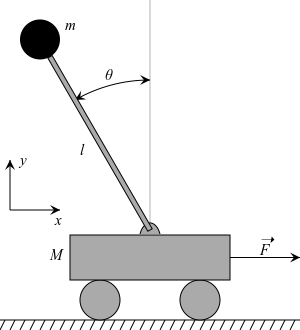
\includegraphics[width=7cm]{images/pendulum.png}
    \caption{The inverted pendulum model}
    \label{fig:pendulum}
\end{figure}

\emph{Consider a cart with an inverted pendulum hinged on top of it as shown in the Figure \ref{fig:pendulum}. For simplicity, the cart and the pendulum are assumed to move in only one plane, and the friction, the mass of the stick, and the gust of wind are disregarded. The problem is to maintain the pendulum at the vertical position. For example, if the inverted pendulum is falling in the direction shown, the cart moves to the right and exerts a force, through the hinge, to push the pendulum back to the vertical position.}\\
\emph{Let's consider the linearized inverted pendulum system (assuming $\theta(t)$ and $\Dot{\theta}(t)$ are very small)}

\begin{equation}
\begin{bmatrix}
    \Dot{x}_1(t) \\ \Dot{x}_3(t) \\ \Dot{x}_3(t) \\  \Dot{x}_4(t) \\ 
\end{bmatrix}
=
\begin{bmatrix}
    0 & 1 & 0 & 0 \\
    0 & 0 & -\frac{mg}{M} & 0 \\
    0 & 0 & 0 & 1 \\
    0 & 0 & \frac{(M+m)g}{Ml} & 0 
\end{bmatrix}
\begin{bmatrix}
    x_1(t) \\ x_2(t) \\ x_3(t) \\ x_4(t)
\end{bmatrix}
+
\begin{bmatrix}
    0 \\ \frac{1}{M} \\ 0 \\ - \frac{1}{Ml}
\end{bmatrix}
u(t)
\end{equation}
\emph{where $x_1(t) = x(t), \smallspace x_2(t) = \Dot{x}(t), \smallspace x_3(t) = \theta(t), \smallspace and \smallspace x_4(t) = \Dot{\theta}(t)$.}\\
\emph{Consider the LQR problem}

\begin{align}
    &u^* := \argmin_{u:[0,\infty) \to \mathbb{R}^m} J(u) := \int_0^\infty \left( x(t)^T Qx(t) + u(t)^T R u(t) \right) dt \\
    &\text{subject to}\\
    &\Dot{x}(t) = Ax(t) + Bu(t), \smallspace x(0) = x_0
\end{align}

\emph{where A and B are appropriate system matrices with m=1, M=2, l=3 and g=9.8.} \\
\emph{Tasks:}

\begin{enumerate}
    \item \emph{Appropriately choose the weighting $Q \geq 0$ and $R > 0$ to maintain the pendulum at the vertical position, i.e., $\theta(t) = 0$ and $\Dot{\theta}(t) = 0$ as much as possible.}
    \item \emph{Find an optimal policy for the LQR problem using Python or Matlab functions.}
    \item \emph{Plot trajectories of the system x(t) and the control input u(t) over certain time interval to demonstrate the performance of your optimal control policy.}
    \item \emph{In the answer, please include your Python or Matlab codes.}
    \item \emph{Change the weight and see how the performance changes and discuss about the results.}
\end{enumerate}
\\
\\
\textbf{Solution:}\\
\\

We want to keep the pendulum in the upright position as much as possible. Therefore, we can choose the values of $Q$ and $R$ as following:
\begin{itemize}
    \item Matrix $Q$: the values on the diagonal of the $Q$ matrix act as "penalties" for the corresponding state variable i.e. we want the $\theta, \dot{\theta}$ as small as possible hence they have a greater penalty. As such, the designed matrix is:
    \begin{equation}
        Q = \begin{bmatrix}
             1 & 0 & 0 &  0\\
             0 & 1 & 0 & 0\\
             0 & 0 & 100 & 0\\
             0 & 0 & 0 & 100\\
        \end{bmatrix}
    \end{equation}
    where the greater values correspond to the \emph{penalties} for $\theta$ and $\dot{\theta}$
    \item Matrix $R$: in this case we just have a uni-dimensional matrix. The larger the $R$ value, the larger the penalty on the input $u(t)$ and therefore the system will use less energy. We set
    \begin{equation}
        R = \begin{bmatrix}
            0.1\\
        \end{bmatrix}
    \end{equation}
\end{itemize}

The Python code for setting the matrices is as following:
\begin{minted}{python}
# Import libraries
import numpy as np
import torch
import scipy.linalg

# Parameters
m = 1 # pendulum mass
M = 2 # cart mass
l = 3 # pendulum length
g = 9.8 # gravity acceleration

# Build matrices
A = np.array([[0, 1, 0, 0], 
              [0, 0, -m*g/M, 0],
              [0, 0, 0, 1], 
              [0, 0, (M+m)*g/(M*l), 0]])
B = np.array([[0], [1/M], [0], [-1/(M*l)]])
rho = 0.1
Q = np.matrix([
    [1, 0, 0,   0],
    [0, 1, 0,   0],
    [0, 0, 100, 0],
    [0, 0, 0, 100]])
R = rho * np.eye(1) # control size is 1
\end{minted}

Then we define the LQR controller as following, where $X$ is the solution to the Riccati equations solved via the Python library \href{https://www.scipy.org/}{SciPy}. The closed loop gain $K$ is then defined as:
\begin{equation}
    K = R^{-1} B^T X
\end{equation}

Python code:
\begin{minted}{python}
def LQR(A,B,Q,R):
    """Solve the continuous time lqr controller.
    dx/dt = A x + B u
    cost = integral x.T*Q*x + u.T*R*u
    """
    #ref Bertsekas, p.151

    # First, try to solve the Riccati equation
    X = np.matrix(scipy.linalg.solve_continuous_are(A, B, Q, R))

    # Compute the LQR gain
    K = np.matrix(scipy.linalg.inv(R)*(B.T*X))

    eigVals, eigVecs = scipy.linalg.eig(A-B*K)

    return K, X, eigVals

K, X, eigVals = LQR(A, B, Q, R)

\end{minted}

By running the code with our designed controller we get:
\begin{equation}
    K = \begin{bmatrix}
        -3.16227766  & -9.26594071 &-146.94265769 & -80.13776765\\
    \end{bmatrix}
\end{equation}
In order to simulate the system, we design a class simulating the inverted pendulum and its physical behavior in time, which is discretized in steps of $\tau = 0.02s$:

\begin{minted}{python}
class ControlledPendulum():
''' Continuous version of the OpenAI Gym cartpole '''
def __init__(self, M, m, l, tau=0.02, g=9.81):
    self.gravity = g
    self.masscart = M
    self.masspole = m
    self.total_mass = (self.masspole + self.masscart)
    self.length = l  # actually half the pole's length
    self.polemass_length = (self.masspole * self.length)
    self.force_mag = 30.0
    self.tau = tau  # seconds between state updates
    self.state = None # Initialize through reset
    
def step(self, force):
    x, x_dot, theta, theta_dot = self.state
    costheta = math.cos(theta)
    sintheta = math.sin(theta)
    temp = (force + self.polemass_length * theta_dot \
        * theta_dot * sintheta)/ self.total_mass
    thetaacc = (self.gravity * sintheta - costheta * temp) / \
        (self.length * (4.0/3.0 - self.masspole * \
        costheta * costheta / self.total_mass))
    xacc = temp - self.polemass_length * thetaacc * \ 
        costheta / self.total_mass
    x = x + self.tau * x_dot
    x_dot = x_dot + self.tau * xacc
    theta = theta + self.tau * theta_dot
    theta_dot = theta_dot + self.tau * thetaacc
    self.state = x, x_dot, theta, theta_dot # save state
    return np.array(self.state, dtype='float64').reshape(4,1)

def reset(self, x_initial= [1, 0, 0, 0], random=False):
    # We can also simulate a disturbance from a random distribution
    if random == True:
        self.state = np.random.uniform(-0.1, 0.1, size=4)
    else:
        self.state = x_initial
    return np.array(self.state, dtype='float64').reshape(4,1)
\end{minted}

We can now start the simulation. We set up the model and set as initial state:
\begin{equation}
    x_0 = \begin{bmatrix}
        1\\
        0\\
        0\\
        0\\
    \end{bmatrix}
\end{equation}

The optimal control input is calculated at each time instant as 
\begin{equation}
    u^*(t) = -K x(t) 
\end{equation}
We simulate $10$ seconds with the following Python code:

\begin{minted}{python}
# Start from position -1 meter
x0 = [-1, 0, 0, 0] 

# Set the model to the initial position
x = model.reset(x_initial=x0, random=False)

# Save trajectory for the graph
trajectory = []
controls = []

# Control loop
for i in range(500):
    u = - K.dot(x)  # the control input is u* = -Kx
    x = model.step(u) # propagate
    trajectory.append(x)
    controls.append(u)
\end{minted}

\paragraph{Position and velocity plots}
We use the following code for plotting: 
\begin{minted}{python}
# Trajectory plotting
import matplotlib.pyplot as plt

tau = 0.02 # time of system update
tot_time = tau*len(trajectory)
t = np.linspace(0, tot_time, len(trajectory)) # time

x_traj, xdot_traj, theta_traj, thetadot_traj, 
    ctrl_traj = [], [], [], [], []
for i in range(len(trajectory)):
    x_traj.append(trajectory[i][0][0])
    xdot_traj.append(trajectory[i][1][0])
    theta_traj.append(trajectory[i][2][0])
    thetadot_traj.append(trajectory[i][3][0])
    ctrl_traj.append(controls[i][0][0].item())
    
fig, ax = plt.subplots(1,1, figsize=(16, 8))
ax.plot(t, x_traj, "k", alpha=.8, label=r'$x(t)$ [$m$]')
ax.plot(t, xdot_traj, "-.k", alpha=.8, label=r'$\dot{x}(t)$ [$m/s$]')
ax.plot([0, tot_time], [0, 0], ":b", alpha=.5, label=r'Setpoint')
ax.legend(loc='upper right')
ax.set_xlabel(r'Time [$s$]')
ax.set_ylabel(r'Value')
ax.set_title("Position and velocity plot")
fig.savefig('images/pendulum_pos_vel.jpg')
\end{minted}
We get the following result:
\begin{figure}[h!]
    \centering
    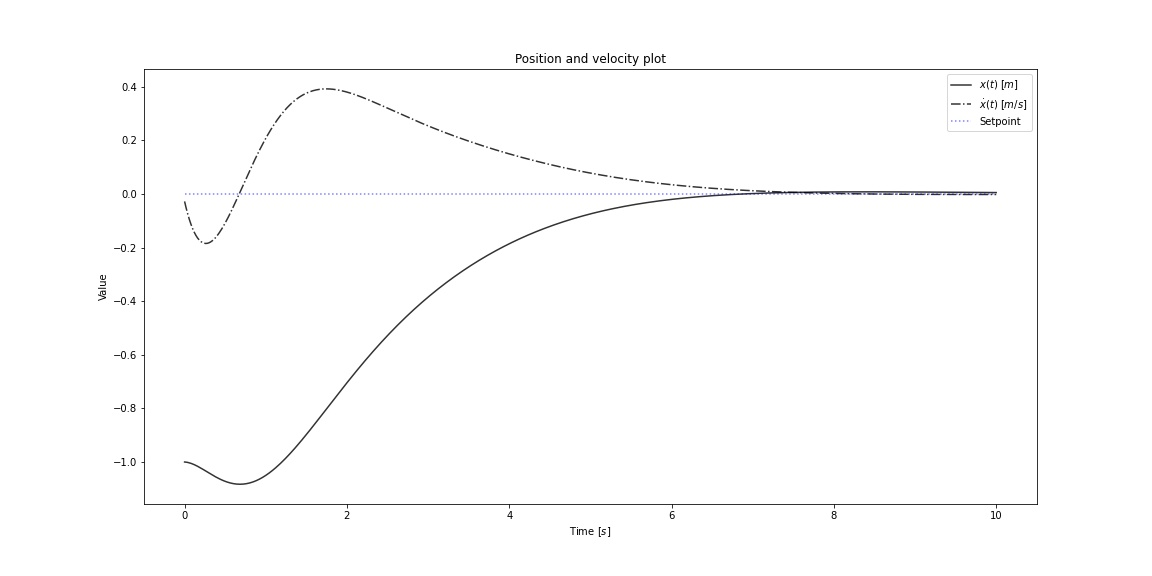
\includegraphics[width=\textwidth]{images/1-pendulum_pos_vel.jpg}
    \caption{Position and velocity plot}
    \label{fig:cartpole_posvel}
\end{figure}
We can see from Figure \ref{fig:cartpole_posvel} that the system is able to stabilize both the position and velocity of the system.

\paragraph{Angular position and angular velocity plots}
Using the following code we obtain
\begin{minted}{python}
fig, ax = plt.subplots(1,1, figsize=(16, 8))
ax.plot(t, theta_traj, "g", alpha=.8,label=r'$ \theta (t)$ [$rad$]')
ax.plot(t, thetadot_traj, "-.g", alpha=.8,label=r'$\dot{ \theta }(t)$ [$rad/s$]')
ax.plot([0, tot_time], [0, 0], ":b", alpha=.5, label=r'Setpoint')
ax.legend(loc='upper right')
ax.set_xlabel(r'Time [$s$]')
ax.set_ylabel(r'Value')
ax.set_title("Angular position and angular velocity plot")
fig.savefig('images/pendulum_angular_pos_vel.jpg')
\end{minted}

\begin{figure}[h!]
    \centering
    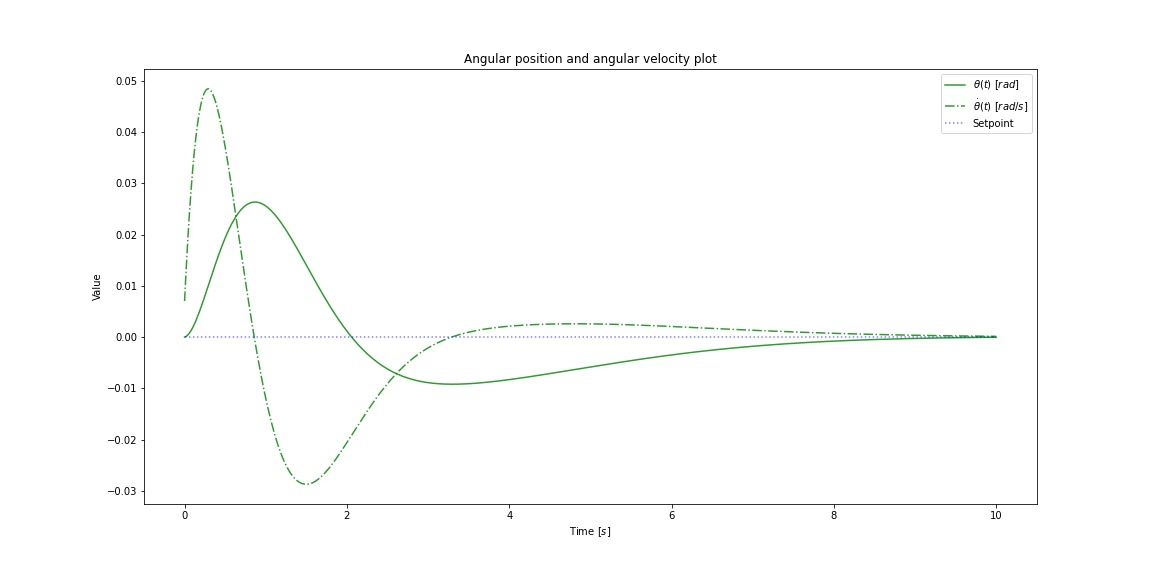
\includegraphics[width=\textwidth]{images/1-pendulum_angular_pos_vel.jpg}
    \caption{Angular positions and velocities}
    \label{fig:cartpole_ang}
\end{figure}

We can infer from Figure \ref{fig:cartpole_ang} that the system is able to stabilize both the angular position and angular velocity of the system and that their values are indeed very close to $0$.

\paragraph{Control input plots}
Using the following code we obtain
\begin{minted}{python}
fig, ax = plt.subplots(1,1, figsize=(16, 8))
ax.plot(t, ctrl_traj, "r", alpha=.6,label=r'$ u^*(t)$ [$N$]')
ax.plot([0, tot_time], [0, 0], ":b", alpha=.5, label=r'Setpoint')
ax.legend(loc='upper right')
ax.set_xlabel(r'Time [$s$]')
ax.set_ylabel(r'Value')
ax.set_title("Control input")
fig.savefig('images/pendulum_input.jpg')
\end{minted}

\begin{figure}[h!]
    \centering
    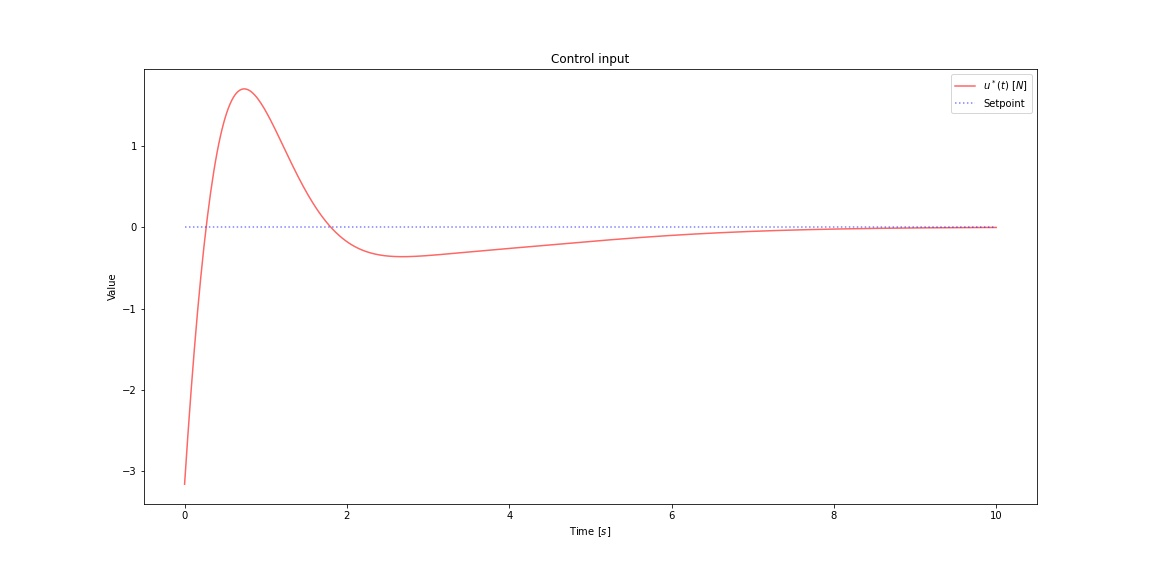
\includegraphics[width=\textwidth]{images/1-pendulum_input.jpg}
    \caption{Control input plot}
    \label{fig:cartpole_input}
\end{figure}

We can see from Figure \ref{fig:cartpole_input} that the system is using a control input $u(t)$ which is able to stabilize the state. Moreover, as expected, $\lim_{t \to \infty} u(t) = 0$.

\paragraph{Changing the weights}
We can now try to change the weights to see how the system performance changes. Let's say we want to penalize the position variation more in order to get a faster stabilization of the position and velocity. We design the matrix $Q$ as: 

\begin{equation}
    Q = \begin{bmatrix}
         100 & 0 & 0 &  0\\
         0 & 100 & 0 & 0\\
         0 & 0 & 100 & 0\\
         0 & 0 & 0 & 100\\
    \end{bmatrix}
\end{equation}

while keeping all the other parameters the same for a fair comparison. We get the control input gain as:
\begin{equation}
    K = \begin{bmatrix}
        -31.6227766  & -69.00397721 & -612.25803618  & -334.32523211\\
    \end{bmatrix}
\end{equation}
By comparison with the previous gain, we notice that the absolute value of the parameters is higher; this will result in a more "aggressive" control.
The plot are the following, in the same order as the experiment before in the below plots.
\begin{figure}[h!]
    \centering
    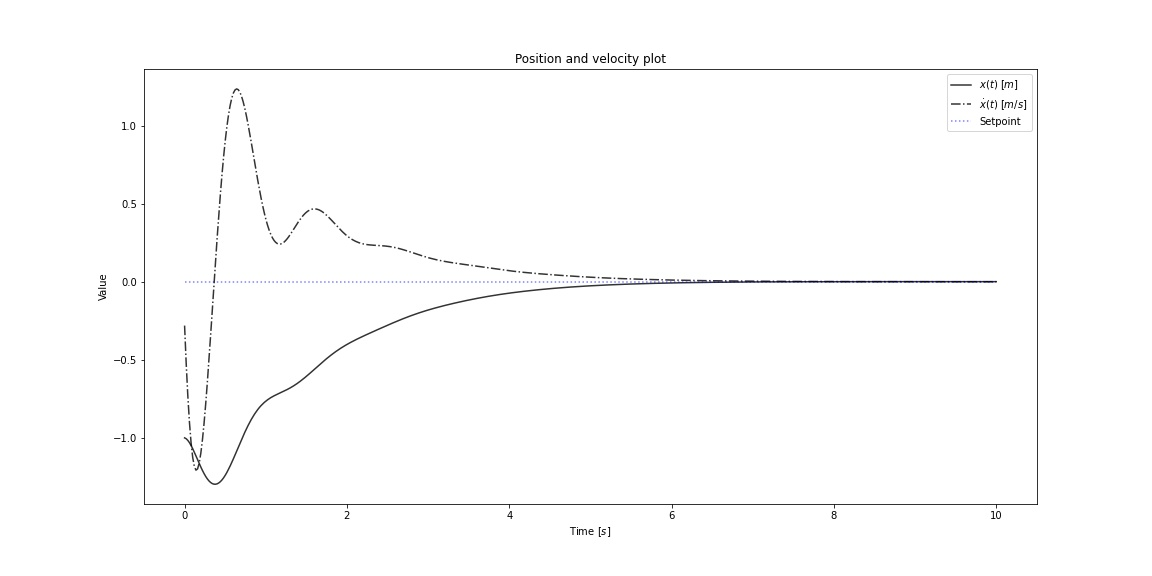
\includegraphics[width=\textwidth]{images/2-pendulum_pos_vel.jpg}
    \label{fig:pen_pos}
    \caption{New position and velocity plot}
\end{figure}
\begin{figure}[h!]
    \centering
    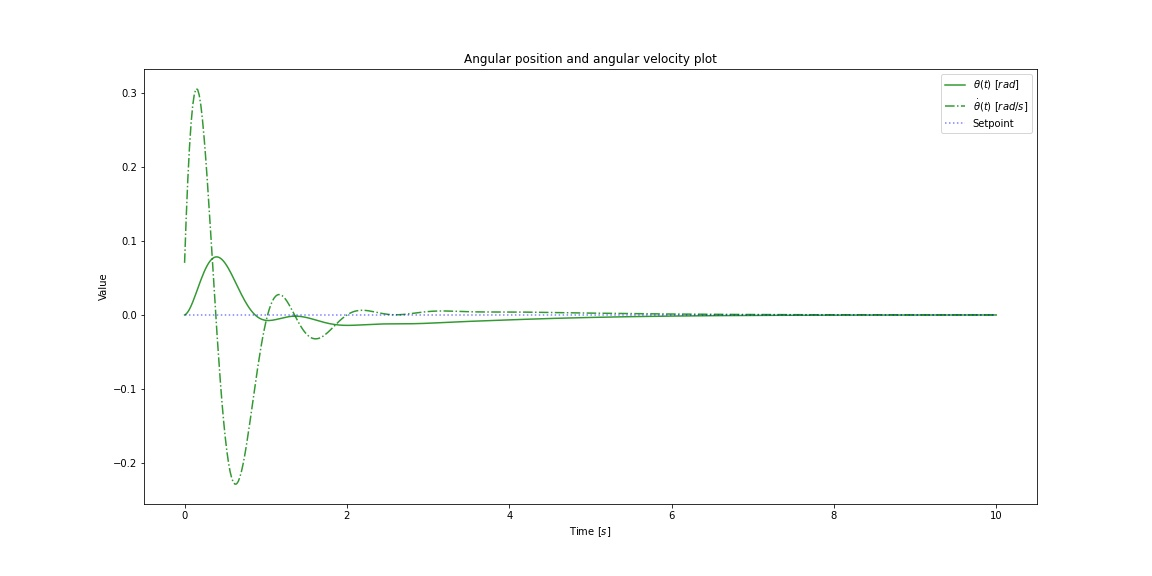
\includegraphics[width=\textwidth]{images/2-pendulum_angular_pos_vel.jpg}
    \label{fig:pen_an}
    \caption{New angular position and angular velocity plot}

\end{figure}
\begin{figure}[h!]
    \centering
    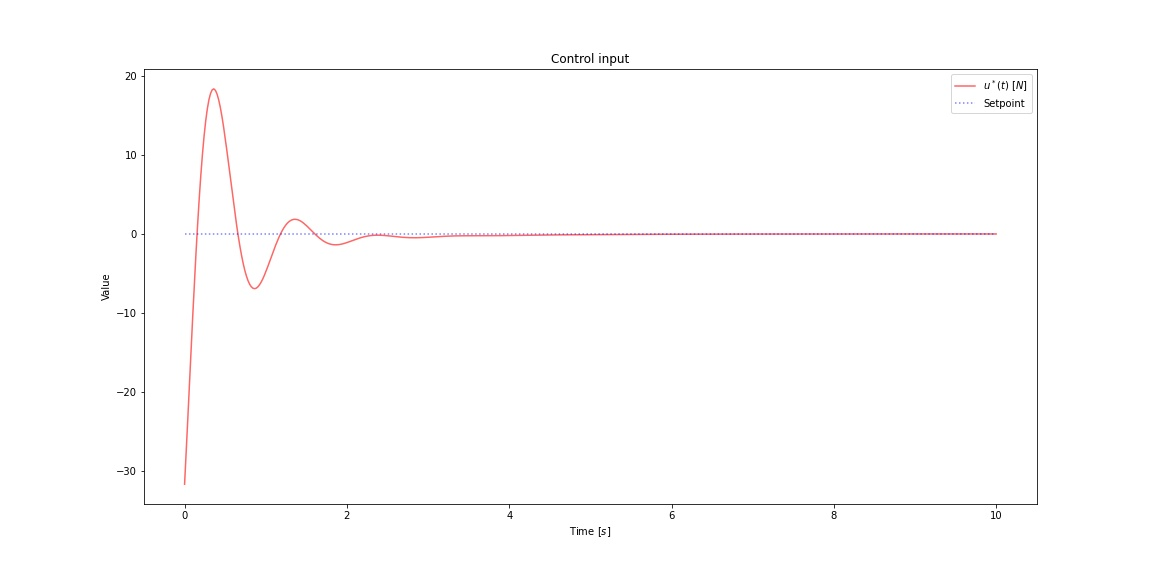
\includegraphics[width=\textwidth]{images/2-pendulum_input.jpg}
    \label{fig:pen_in}
    \caption{New control input plot}
\end{figure}

These results confirm our hypothesis: the position and velocity stabilize faster, at the cost of a higher variation for the angular position and velocity. Moreover, since the weight for the control input was chosen as $0.1$, its absolute value is much larger than before; the first was in the range of $u(t) \in (-4, 2)$ while the new control input has a much wider range around $u(t) \in (-40, 20)$. Thus, a more aggressive controller results in using more energy for a faster stabilization.